\chapter{Regression and Reconstruction on Cartesian Product Graphs} 

\label{chap:reg_and_rec} 

\lhead{Chapter 4. \emph{Regression and Reconstruction on Cartesian Product Graphs}} 


 
\section{Graph Products}

\label{sec:reg_and_rec_intro}

In this chapter, we turn our attention to the topic of signal processing on \textit{Cartesian product graphs}. This special class of graph finds applications in numerous areas, such as video, hyper-spectral image processing and network time series problems. However, the Cartesian product is not the only way to consistently define a product between two graphs. In this section we formally introduce the concept of a graph product, examine  some prominent examples, and explain why we choose to look specifically at the Cartesian graph product. 

\subsection{Basic definitions}

In the general case, consider two undirected graphs $\mathcal{G}_A = (\mathcal{V}_A, \mathcal{E}_A)$ and $\mathcal{G}_B = (\mathcal{V}_B, \mathcal{E}_B)$ with vertex sets given by $\mathcal{V}_A = \{a \in \mathbb{N} \, | \, a \leq A \}$ and $\mathcal{V}_B = \{b \in \mathbb{N} \, | \, b \leq B \}$ respectively. (In this context we do not regard zero to be an element of the natural numbers). A new graph $\mathcal{G}$ can be constructed by taking the product between $\mathcal{G}_A$ and $\mathcal{G}_B$. This can be generically written as follows. 

\begin{equation}
    \mathcal{G} = \mathcal{G}_A \, \diamond \, \mathcal{G}_B = (\mathcal{V}, \, \mathcal{E})
\end{equation}

For all definitions of a graph product, the new vertex set $\mathcal{V}$ is given by the Cartesian product of the vertex sets of the factor graphs, that is
 
\begin{equation}
    \mathcal{V} = \mathcal{V}_A \times \mathcal{V}_B = \{(a, \, b) \in \mathbb{N}^2 \, | \, a \leq A \; \text{and} \; b \leq B \}
\end{equation}


Typically, vertices are are arranged in lexicographic order, in the sense that $(a, \, b) \leq (a',\, b')$ iff $a < a'$ or ($a = a'$ and $b \leq b'$) \citep{Harzheim2005}. Each consistent rule for constructing the new edge set $\mathcal{E}$ corresponds to a different definition of a graph product. In general, there are eight possible conditions for deciding whether two nodes $(a, \, b)$ and $(a',\,  b')$ are to be connected in the new graph.

% visual? 


\begin{table}[h]
\def\arraystretch{1.5}
\centering
\begin{tabular}{lclc}
1. & $[a, \, a'] \in \mathcal{E}_A$ & and &  $b = b'$  \\
2. & $[a, \, a'] \notin \mathcal{E}_A$  & and &  $b = b'$  \\
3. & $[a, \, a'] \in \mathcal{E}_A$ & and &  $[b, \, b'] \in \mathcal{E}_B$ \\
4. & $[a, \, a'] \notin \mathcal{E}_A$ & and &  $[b, \, b'] \in \mathcal{E}_B$  \\
5. & $[a, \, a'] \in \mathcal{E}_A$ & and & $[b, \, b'] \notin \mathcal{E}_B$  \\
6. & $[a, \, a'] \notin \mathcal{E}_A$ & and & $[b, \, b'] \notin \mathcal{E}_B$  \\
7. & $a = a'$ & and & $[b, \, b'] \in \mathcal{E}_B$,  \\
8. & $a = a'$ & and &  $[b, \, b'] \notin \mathcal{E}_B$ 
\end{tabular}
\end{table}



Each definition of a graph product corresponds to the union of a specific subset of these conditions, thus, there exist 256 different types of graph product \citep{Barik2015}. Of these, the Cartesian product (conditions 1 or 7), the direct product (condition 3), the strong product (conditions 1, 3 or 7) and the lexicographic product (conditions 1, 3, 5 or 7) are referred to as the standard products and are well-studied \citep{Imrich2000}. A graphical depiction of the standard graph products is shown in figure \ref{fig:graph_products}. In each of these four cases, the adjacency and Laplacian matrices of the product graph can be described in terms of matrices relating to the factor graphs \citep{Fiedler1973, Barik2018}. This is shown in table \ref{tab:grap_product_matrices}. 

\begin{table}[h]
\def\arraystretch{1.8}
\centering
\small
\vspace{0.5cm}
\begin{tabular}{|l|cc|}
    \hline 

    & Adjacency matrix
    & Laplacian \\

    \hline

    Cartesian 
    & $\A_A \oplus \A_B$ 
    & $\LL_A \oplus \LL_B$ \\

    Direct 
    & $\A_A \otimes \A_B$  
    & $\D_A \otimes \LL_B + \LL_A \otimes \D_B - \LL_A \otimes \LL_B$ \\
    
    Strong 
    & $\A_A \otimes \A_B + \A_A \oplus \A_B$ 
    & $\D_A \otimes \LL_B + \LL_A \otimes \D_B - \LL_A \otimes \LL_B + \LL_A \oplus \LL_B$ \\

    Lexicographic 
    & $\I_A \otimes \A_B + \A_A \otimes \J_A$ 
    &  $\I_A \otimes \LL_B + \LL_A \otimes \J_B + \D_A \otimes (|\mathcal{V}_B| \I_B - \J_B)$ \\

    \hline

\end{tabular}
\vspace{0.2cm}
\caption[The adjacency and Laplacian matrices for the standard graph products]{The adjacency and Laplacian matrices for the standard graph products. Here, $\D_A$ and $\D_B$ are the diagonal degree matrices, i.e $\D_A = \diag{\A_A \mathbf{1}}$. $\I_A$ and $\J_A$ are the $(A \times A)$ identity matrix and matrix of ones respectively. } 
\vspace{0.3cm}
\label{tab:grap_product_matrices}
\end{table}

\begin{figure}[t]
    \begin{center}
    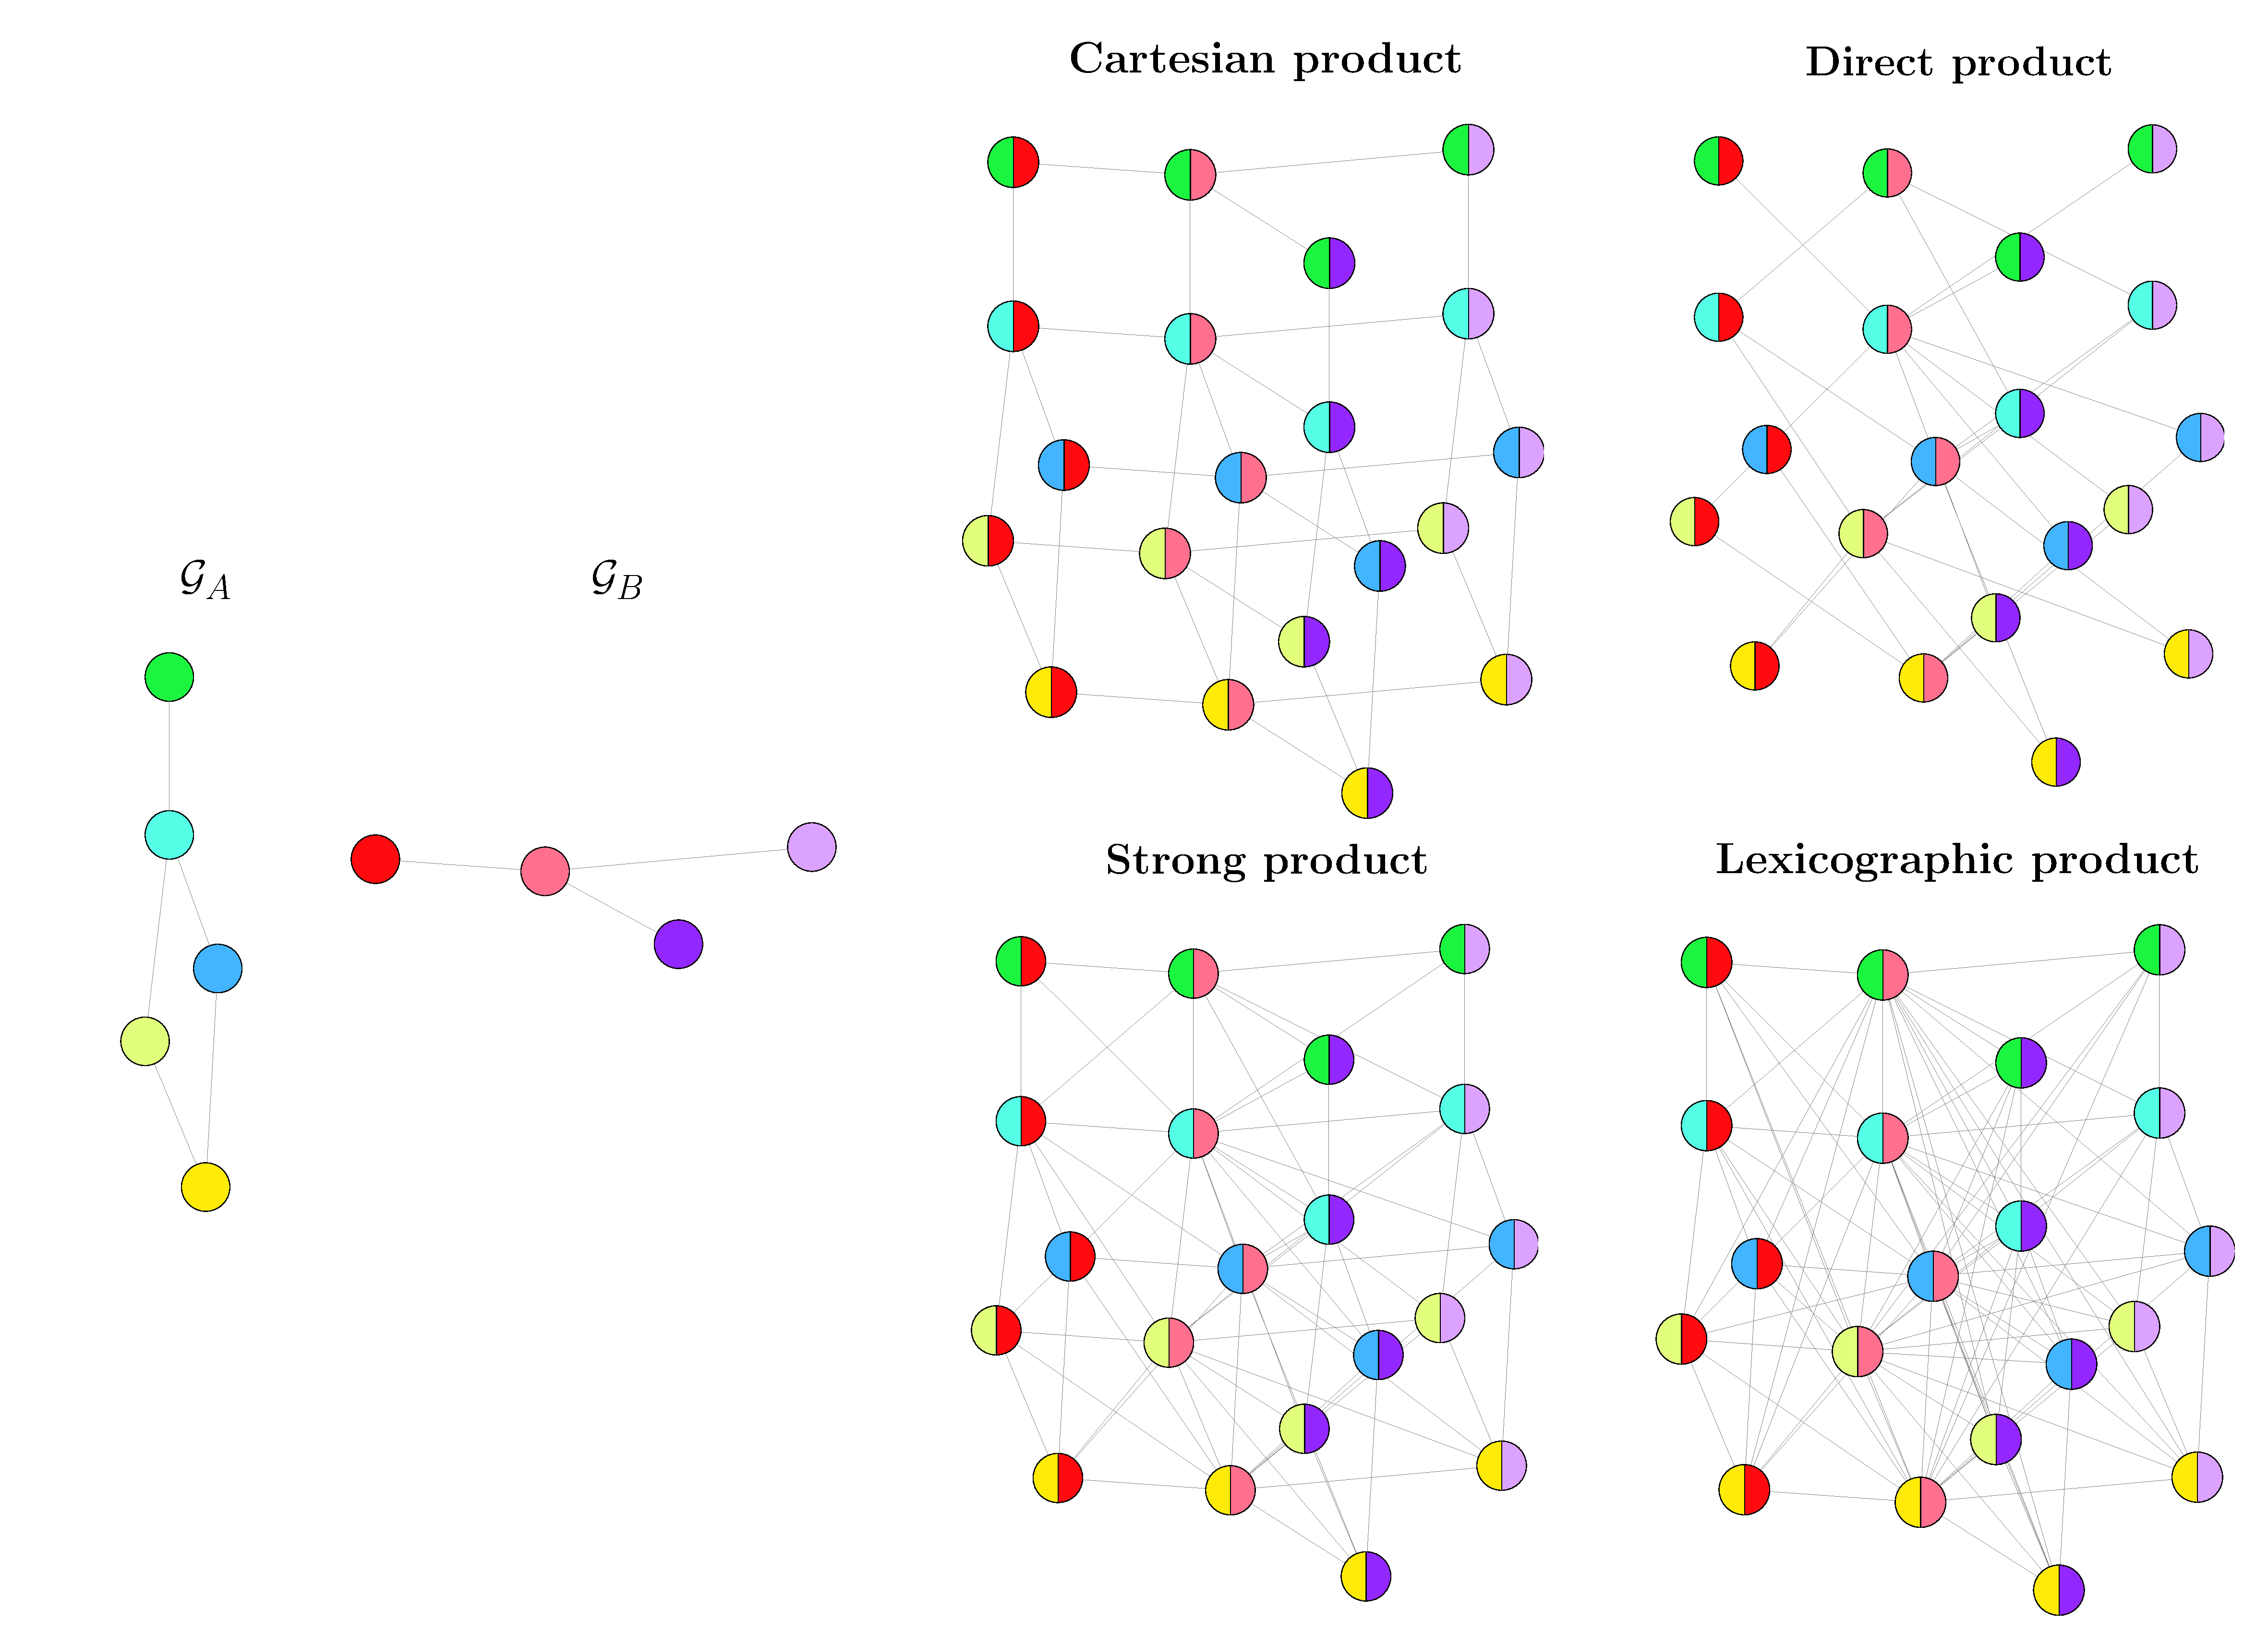
\includegraphics[width=\linewidth]{Figures/product_graphs.pdf}
    \end{center}
    \caption[Graphical depiction of the standard graph products]{A graphical depiction of the four standard graph products}
    \label{fig:graph_products}
\end{figure}

% choice of product effect the sparsity or A/cardinality of V

% What is the natural 256 ordering in terms of sparsity

% make small example in terms of vertex order

Given these definitions, it may seem that all the standard graph products are non-commutative in the sense that $\A_A \oplus \A_B  \neq \A_B \oplus \A_A $ etc. However, the graphs $\mathcal{G}_A \, \diamond \, \mathcal{G}_B$ and $\mathcal{G}_B \, \diamond \, \mathcal{G}_A$ are in fact isomorphically identical in the case of the Cartesian, direct and strong products. This is not the case for the Lexicographic product \citep{Imrich2000}. 

\subsection{The spectral properties of graph products}

In the field of graph signal processing, we are often concerned with analysing the properties of graphs via eigendecomposition of the graph Laplacian \citep{Mieghem2010}. In the case of product graphs, it is greatly preferable if we are able to fully describe the spectrum of $\mathcal{G}_A \diamond \mathcal{G}_B$ in terms of the spectra of $\mathcal{G}_A$ and $\mathcal{G}_B$ alone. This is because direct decomposition of a dense $\LL$ has time-complexity $O(A^3B^3)$, whereas decomposition of the factor Laplacians individually has complexity $O(A^3 + B^3)$. As the graphs under considerations become medium to large, this fact quickly makes direct decomposition of the product graph Laplacian intractable. However, in the general case, only the spectra of the Cartesian and lexicographic graph products can be described in this way \citep{Barik2018}. In the case of the direct and strong product, it is possible to estimate the spectra without performing the full decomposition (see \citep{Sayama2016}). However, in general, the full eigendecomposition of the product graph Laplacian can only be described in terms of the factor eigendecompositions when both factor graphs are regular. 


Consider the eigendecompositions of $\LL_A$ and $\LL_B$. 

\begin{equation}
    \LL_A = \U_A \LAM_A \U_A^\top, \aand \LL_B = \U_B \LAM_B \U_B^\top
\end{equation}

where $\U_A$ and $\U_B$ are the respective orthonormal eigenvector matrices, and $\LAM_A$ and $\LAM_B$ are the diagonal eigenvalue matrices given by 

\begin{equation}
    \LAM_A = \begin{bmatrix}
        \lambda_1^{(A)}, & & & \\
        & \lambda_2^{(A)} & & \\
        & & \ddots & \\
        & & & \lambda_A^{(A)} \\
    \end{bmatrix}  
    \aand 
    \LAM_B = \begin{bmatrix}
        \lambda_1^{(B)}, & & & \\
        & \lambda_2^{(B)} & & \\
        & & \ddots & \\
        & & & \lambda_B^{(B)} \\
    \end{bmatrix}  
\end{equation}

Given these definitions, table \ref{tab:product_graph_spectra} gives information about the spectral decomposition of the standard graph products.


\begin{table}[h]
    \def\arraystretch{1.8}
    \centering
    \small
    \vspace{0.5cm}
    \begin{tabular}{|l|cc|}
        \hline 
    
        & Eigenvalues
        & Eigenvectors \\
    
        \hline
    
        Cartesian 
        & $\lambda_a^{(A)} + \lambda_b^{(B)}$ 
        & $(\U_A)_a \otimes (\U_B)_b$ \\
    
        Direct$^{\star}$
        & $r_A \lambda_b^{(B)} + r_B \lambda_a^{(A)} - \lambda_a^{(A)} \lambda_b^{(B)}$  
        & $(\U_A)_a \otimes (\U_B)_b$ \\
        
        Strong$^{\star}$
        & $(1+r_A) \lambda_b^{(B)} + (1+r_B) \lambda_a ^{(A)}- \lambda_a^{(A)} \lambda_b^{(B)}$
        & $(\U_A)_a \otimes (\U_B)_b$ \\
    
        \multirow{2}{7em}{Lexicographic$^\dagger$}
        & $B \lambda_a^{(A)}$ 
        & $(\U_A)_a \otimes \mathbf{1}_B$ \\

        & $\lambda_b^{(B)} + B \text{deg}(a)$ 
        & $\mathbf{e}_a \otimes (\U_B)_b$  \\
    
        \hline
    
    \end{tabular}
    \vspace{0.2cm}
    \caption[Spectral decomposition of product graphs]{Eigendecomposition of the Laplacian of the standard graph products. Here, $a$ and $b$ are understood to run from 1 to $A$ and 1 to $B$ respectively. $\star$ only for $r_A$ and $r_B$-regular factor graphs. $\dagger$ note that the $b$ runs from 2 to $B$ in the lower row. } 
    \vspace{0.3cm}
    \label{tab:product_graph_spectra}
    \end{table}
    
% remark common degree locally only necessary 
% subspace concentration 


\subsection{GSP with Cartesian product graphs} 

While both the direct and strong products do find uses in certain applications (for example, see \citep{Kaveh2011}), they are both less common and more challenging to work with in a graph signal processing context due to their spectral properties described in the previous subsection. In practice, being limited to regular factor graphs means the majority of practical GSP applications are ruled out. The lexicographic product does not share this drawback, however it is also significantly less common than the Cartesian product in real-world applications. For this reason, in the following, we focus primarily on the Cartesian product. 

Given the spectral decomposition of the Cartesian graph product stated in table \ref{tab:product_graph_spectra}, we can write the Laplacian eigendecomposition in matrix form as follows. 

\begin{equation}
    \LL = \U \LAM \U^\top, \where \U = \U_A \otimes \U_B \aand \LAM = \LAM_A \oplus \LAM_B
\end{equation}

This motivates the following definitions for the Graph Fourier Transform (GFT) and its inverse (IGFT). Consider a signal defined over the nodes of a Cartesian product graph expressed as a matrix $\Y \in \R^{B \times A}$. We can perform the GFT as follows. 

% when is this well-defined? 
% FFT version?
% impose statements on the properties of Y
% stationarity? 


\begin{equation}
    \text{GFT}(\Y) = \MAT{\big( \U_A^\top \otimes \U_B^\top \big) \, \vecc{\Y}} = \U_B^\top \Y \U_A
\end{equation}

Correspondingly, we can define the IGFT acting on a matrix of spectral components $\Z \in \R^{B \times A}$ as follows. 

\begin{equation}
    \text{IGFT}(\Z) = \MAT{\big( \U_A \otimes \U_B \big)\,\vecc{\Z}} = \U_B \Z \U_A^\top
\end{equation}


\note{Product graph signals: repseprentation and vectorisation}{

    It is natural to assume that signals defined on the nodes of a Cartesian product graph $\mathcal{G}_A \, \square \; \mathcal{G}_B$ could be represented by matrices (order two tensors) of shape $(A \times B)$. Since product graph operators, such as the Laplacian $\LL_A \oplus \LL_B$, act on vectors of length $AB$, we must define a consistent function to map matrix graph signals $\in \R^{A \times B}$ to vector graph signals $\in \R^{AB}$. The standard mathematical operator for this purpose is the $\vecc{\cdot}$ function, along with its reverse operator $\mat{\cdot}$. However, this is somewhat problematic since $\vecc{\cdot}$ is defined to act in \textit{column-major} order, that is 

    $$
    \text{vec} \left( \begin{bmatrix}
        \Y_{(1, 1)} & \Y_{(1, 2)} & \dots & \Y_{(1, B)} \\
        \Y_{(2, 1)} & \Y_{(2, 2)} & \dots  & \Y_{(2, B)} \\
        \vdots & \vdots & \ddots & \vdots \\
        \Y_{(A, 1)} & \Y_{(A, 2)} & \dots  & \Y_{(A, B)} \\
    \end{bmatrix} \right) 
    =
    \begin{bmatrix}
        \Y_{(1, 1)} \\ \Y_{(2, 1)} \\ \vdots \\ \Y_{(A-1, B)} \\ \Y_{(A, B)}
    \end{bmatrix}
    $$

    As is visible, this does not result in a lexicographic ordering of the matrix elements when the graph signal has shape $(A \times B)$. Therefore, to avoid this issue and to be consistent with standard mathematical notation, we will assume that graph signals are represented by matrices  of shape $(B \times A)$ when considering the product between two graphs $\mathcal{G}_A \, \square \, \mathcal{G}_B$. For graph signals of this shape, the first index represents traversal of the nodes in $\mathcal{G}_B$, and the second index represents traversal of the nodes in $\mathcal{G}_A$. This ensures that matrix elements are correctly mapped to vector elements when using the column-major $\vecc{\cdot}$ function. 

}

Given these definitions, we can define a spectral operator (usually a low-pass filter) $\HH$ which acts on graph signals according to a spectral scaling function $g(\lambda \,; \, \beta)$ such as one of those defined in table \ref{tab:iso_filters}. As with regular non-product graphs, the action of this operator can be understood as first transforming a signal into the frequency domain via the GFT, then scaling the spectral components according to some function, and finally transforming back into the vertex domain via the IGFT. 

\begin{align} 
    \label{eq:graph_filter}
    \HH &= g(\LL_A \oplus \LL_B) \notag \\ 
       &= \big( \U_A \otimes \U_B \big) \, g \big( \LAM_A \oplus \LAM_B \big) \, \big( \U_A^\top \otimes \U_B^\top \big) \notag \\
       &= \big( \U_A \otimes \U_B \big) \, \Diag{\vecc{\G}} \, \big( \U_A^\top \otimes \U_B^\top \big)
\end{align}

% remark which section of the thesis the properties of G are explained

The matrix $\G \in \R^{B \times A}$, which we refer to as the spectral scaling matrix, holds the value of the scaling function applied to the sum of
pairs of eigenvalues, such that

\begin{equation}
    \G_{ba} = g(\lambda^{(A)}_a + \lambda^{(B)}_b; \beta)
\end{equation}

 
% remark about Cartesian product eig sum

We observe that defining the filtering operation in this manner implies that the intensity is equal across both $\mathcal{G}_A$ and $\mathcal{G}_B$. We refer to filters of this type as \textit{isotropic}. This can be further generalised by considering an \textit{anisotropic} graph filter, which offers independent control over the filter intensity in each of the two dimensions. In this case, we define $\G$ as follows. 

\begin{equation}
    \G_{ba} =  g \left( \begin{bmatrix}
        \lambda^{(A)}_a \\ \lambda^{(B)}_b 
    \end{bmatrix}, \; \begin{bmatrix}
        \beta_a \\ \beta_b 
    \end{bmatrix} \right)
\end{equation}

where now $g(\lambdaa \,; \, \betaa)$ is chosen to be an anisotropic graph filter such as one of those listed in table \ref{tab:anis_filters}. Note that the original parameter $\beta$ is now replaced by a vector of parameters $\betaa$ which control the filter intensity in each dimension. 

\begin{figure}[b]
    % \begin{center}
    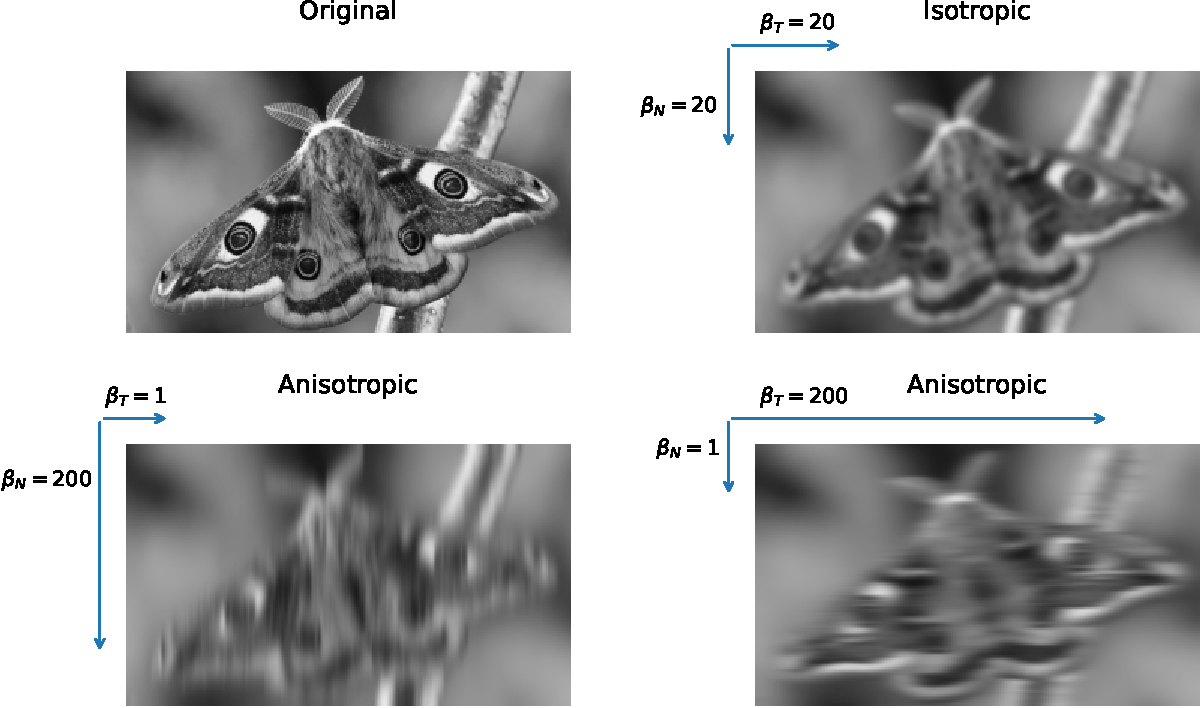
\includegraphics[width=0.9\linewidth]{Figures/filter_types_butterfly.pdf}
    % \end{center}
    \caption[A time-vertex Cartesian product graph]{A graphical depiction of a time-vertex Cartesian product graph}
    \label{fig:TV}
\end{figure}
 
\begin{table}[t]
    \def\arraystretch{1.7}
    \small
    \begin{center}
    \begin{tabular}{|l|c|}
    \hline
    \textbf{Filter}   & $g(\lambdaa; \,\betaa)$    \\ 
    \hline
    1-hop random walk & $(1 + \betaa^\top\lambdaa)^{-1}$ \\
    \hline
    Diffusion         & $\exp(-\betaa^\top\lambdaa)$       \\
    \hline
    ReLu              & $\max (1 - \betaa^\top\lambdaa, 0)$  \\
    \hline
    Sigmoid           & $2 \big( 1 + \exp(\betaa^\top\lambdaa)\big)^{-1}$ \\
    \hline
    Bandlimited       & $1, \,\text{if} \; \betaa^\top\lambdaa \leq 1 \; \text{else} \; 0$   \\
    \hline
    \end{tabular}
    \end{center}
    \caption{Anisotropic graph filter functions}
    \label{tab:anis_filters}
    \end{table}



\section{Graph Signal Reconstruction on Cartesian Product Graphs}

\label{sec:gsr_cpg}

We now turn our attention to the task of signal reconstruction on Cartesian product graphs. In the following, we will replace the factor graph labels $A$ and $B$ with $T$ and $N$ respectively. The reason for this is that one application of particular interest is graph time-series problems, where we seek to model a network of $N$ nodes across a series of $T$ discrete time points. These so called ``time-vertex'' (T-V) problems have garnered significant interest recently in the context of GSP \citep{Grassi2018, Isufi2017, Loukas2016}. T-V signals can be understood as existing on the nodes of a Cartesian product graph $\mathcal{G}_T \, \square \, \mathcal{G}_N$. In particular, we can conceptualise $T$ repeated measurements of a signal defined across the nodes of a $N$-node graph as a single measurement of a signal defined on the nodes of $\mathcal{G}_T \, \square \, \mathcal{G}_N$, where $\mathcal{G}_T$ is a simple path graph.

\vspace{1cm}


\begin{figure}[b]
    \begin{center}
    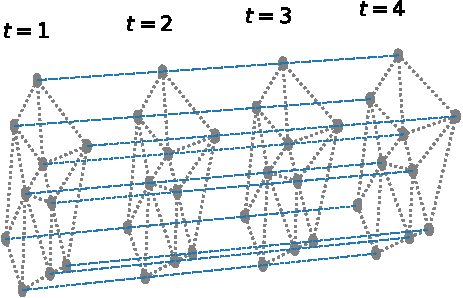
\includegraphics[width=0.5\linewidth]{Figures/T-V.pdf}
    \end{center}
    \caption[A time-vertex Cartesian product graph]{A graphical depiction of a time-vertex Cartesian product graph}
    \label{fig:TV}
\end{figure}



\note{On the Laplacian spectrum of the path graph}{
    When considering time-vertex problems, $\mathcal{G}_T$ will generally be described by a  path graph. This special case of a graph has vertices given by $\mathcal{V}_T = \{t \in \mathbb{N} \, | \, t \leq T \}$ and edges given by $\mathcal{E}_T = \{ \, [t, t+1] \, | \, t < T \}$. The Laplacian matrix of the path graph is therefore given by 

    $$
    \LL_T = \begin{bmatrix}
        1 & -1 & & & \\
        -1 & 2 & -1 & &   \\
        & & \ddots & &   \\
        & &  -1 & 2 & -1 \\
        & & &  -1 & 1 \\
    \end{bmatrix}
    $$

    The eigenvalues and eigenvectors of this Laplacian are well-known and can be expressed in closed-form \citep{Jiang2012}. In particular, 

    $$
    \lambda^{(T)}_t = 2 - 2 \cos \Big(  \, \frac{t - 1}{T} \pi \, \Big)
    $$

    and 

    $$
    (\U_T)_{ij} = \cos \Big( \, \frac{j - 1}{T}\big(i - 0.5\big)\pi \, \Big)
    $$

    % link between this and FFT?

    ($\U_T$ should be appropriately normalised after this computation to ensure each column is orthonormal). Computing the eigendecomposition directly in this fashion reduces the complexity from $O(T^3)$ to $O(T^2)$ which can be significant for large time-series problems. 
 
}

Note that, despite the observation that $\mathcal{G}_T$ is often a path graph in the context of T-V problems, the methods introduced in this section are valid for the Cartesian product between arbitrary undirected factor graphs. 

\subsection{Problem statement}


The goal of Graph Signal Reconstruction (GSR) is to estimate the value of a partially observed graph signal at nodes where no data was collected. In the context of GSR on a Cartesian product graph, the available data is an observed signal $\Y \in \R^{N \times T}$ where only a partial set $\mathcal{S} = \{(n_1, t_1), (n_2, t_2), \dots \}$ of the signal elements were recorded. All other missing elements of $\Y$ are set to zero. Our model is based on the assumption that $\Y$ is a noisy partial observation of an underlying signal $\F \in \R^{N \times T}$, which is itself assumed to be smooth with respect to the graph topology. 

We define the statistical model for the generation of an observation matrix $\Y$ as 

\begin{equation}
    \Y = \Ss \circ \big(\F + \E \big)
\end{equation}

where $\Ss \in [0, 1]^{N \times T}$ is referred to as the sensing matrix, and has entries given by 

\begin{equation}
    \Ss_{nt} = \begin{cases}
        1 & \text{if} \;\; (n, t) \in \mathcal{S} \\
        0 & \text{otherwise}
    \end{cases}
\end{equation}

The matrix $\E$ represents the model error and is assumed to have an independent normal distribution with unit variance. Therefore, the probability distribution of $\Y$ given the latent signal $\F$ is

\begin{equation}
    \label{eq:Y_given_F}
    \vecc{\Y} \, | \, \F \sim \mathcal{N}\Big(\vecc{\Ss \circ \F}, \; \Diag{\vecc{\Ss}}\Big)
\end{equation}

Note that the covariance matrix $\Diag{\vecc{\Ss}}$ is semi-positive definite by construction. This naturally reflects the constraint that some elements of $\Y$ are zero with probability 1. In order to estimate the latent signal $\F$, we must provide a prior distribution describing our belief about its likely profile ahead of time. In general, we expect $\F$ to be smooth with respect to the topology of the graph. This can be expressed by setting the covariance matrix in its prior to be proportional to $\HH^2$, where $\HH$ is a graph filter as defined in equation (\ref{eq:graph_filter}). For now, in the absence of any further information, we assume that the prior mean for $\F$ is zero across all elements. 

\begin{equation}
    \label{eq:F_prior}
    \vecc{\F} \sim \mathcal{N}\big(\mathbf{0}, \, \gamma^{-1} \HH^2\big) 
\end{equation}

Next, given an observation $\Y$, we use Bayes' rule to find the posterior distribution over $\F$. This is given by

\begin{equation}
    \pi\big(\vecc{\F} \, | \, \Y \big) = \frac{\pi\big(\vecc{\Y} \, | \, \F \big) \pi(\F) }{\pi(\Y)}.
\end{equation}

where we use the notation $\pi(\cdot)$ to denote a probability density function.

\begin{theorem}
    The posterior distribution for $\F$ is given by 

    \begin{equation}
        \label{eq:F_post}
            \Vecc{\F} \, | \, \Y \sim \mathcal{N} \big(\SIG \, \Vecc{\Y}, \; \SIG \big)
        \end{equation}
        
        \noindent where 
        
        \begin{equation}
        \label{eq:Sig_post}
            \SIG = \Big(\Diag{\vecc{\Ss}} + \gamma  \HH^{-2}\Big)^{-1}
        \end{equation}

\end{theorem}

\begin{proof}
    Consider the matrix $\Ss_{\epsilon}$ defined in the following manner. 
    
    \begin{equation}
        (\Ss_{\epsilon})_{nt} = \begin{cases}
            1 & \text{if} \;\; (n, t) \in \mathcal{S} \\
            \epsilon & \text{otherwise}
        \end{cases}
    \end{equation}

    We can use this definition to rewrite equation \ref{eq:Y_given_F} for the probability distribution of $\Y | \F$.

    \begin{equation}
        \Vecc{\Y} \, | \, \F \, \sim \, \lim_{\epsilon \rightarrow 0} \, \Bigg[ \, \mathcal{N}\Big(\vecc{\Ss_{\epsilon} \circ \F}, \; \Diag{\vecc{\Ss_{\epsilon}}}\Big) \, \Bigg]
    \end{equation}

    In this way, the negative log-likelihood of an observation $\Y | \F$ is given by 

    \begin{equation}
        \label{eq:log_prob_1}
        - \log \pi(\Y | \F) = \lim_{\epsilon \rightarrow 0} \, \Bigg[  \frac{1}{2} \vecc{\Ss_{\epsilon} \circ \F - \Y}^\top \Diag{\vecc{\Ss_{\epsilon}}}^{-1} \vecc{\Ss_{\epsilon} \circ \F - \Y}\, \Bigg]
    \end{equation}

    up to an additive constant which does not depend on $\F$. Note that, since $\Y = \Ss_{\epsilon}  \circ \Y$, we can rewrite $\vecc{\Ss_{\epsilon} \circ \F - \Y}$ as 

    \begin{align}
        \vecc{\Ss_{\epsilon} \circ \F - \Y} &= \Vecc{\Ss_{\epsilon} \circ  (\F - \Y)}  \notag \\
        &= \Diag{\vecc{\Ss_{\epsilon}}} \vecc{\F - \Y}
    \end{align}

    Therefore, equation \ref{eq:log_prob_1} can be rewritten as 

    \begin{align}
        - \log \pi(\Y | \F) &= \lim_{\epsilon \rightarrow 0} \, \Bigg[  \frac{1}{2} \vecc{\F - \Y}^\top \Diag{\vecc{\Ss_{\epsilon}}} \, \vecc{\F - \Y}\, \Bigg] \notag \\[0.2cm]
        &= \frac{1}{2} \vecc{\F - \Y}^\top \Diag{\vecc{\Ss}} \, \vecc{\F - \Y}
    \end{align}

    Now consider the full log-posterior. Using Bayes rule, this can be written as 

    \begin{multline}
        -\log \pi\big(\vecc{\F} \, | \, \Y \big) = \frac{1}{2} \vecc{\F - \Y}^\top \Diag{\vecc{\Ss}} \, \vecc{\F - \Y} \; + \\ \frac{\gamma}{2} \vecc{\F }^\top\HH^{-2} \, \vecc{\F}
    \end{multline}

    Up to an additive constant not dependent $\F$, this can be written as 

    \begin{equation}
        -\log \pi\big(\vecc{\F} \, | \, \Y \big) = \frac{1}{2} \Big( \vecc{\F}^\top \big( \Diag{\vecc{\Ss}} + \gamma \HH^{-2}\big) \vecc{\F} - 2 \, \vecc{\Y}^\top \F \Big)
    \end{equation}

    Using the conjugacy of the normal distribution, by direct inspection we can conclude that the posterior covariance is given by 

    \begin{equation}
        \SIG = \Big( \Diag{\vecc{\Ss}} + \gamma \HH^{-2} \Big)^{-1}
    \end{equation}

    and that the posterior mean is given by $\SIG \, \vecc{\Y}$. 

\end{proof}

In this chapter, we are primarily interested in computing the posterior mean, which is the solution to the following linear system. 

\begin{equation}
    \label{eq:lin_system}
        \Big(\Diag{\vecc{\Ss}} + \gamma  \HH^{-2}\Big) \, \vecc{\F} = \vecc{\Y}
    \end{equation}

We return to the question of sampling from the posterior and estimating the posterior covariance directly in \cref{chap:variance}. 

Two significant computational challenges arise when working with non-trivial graph signal reconstruction problems, where the number of vertices in the product graph is large. First, although the posterior mean point estimator given in \cref{eq:lin_system} has an exact closed-form solution, its evaluation requires solving an $NT \times NT$ system of equations, which is impractical for all but the smallest of problems. Second, since the eigenvalues of $\HH$ can be close to or exactly zero, $\HH^{-2}$ may be severely ill-conditioned and even undefined. This means the condition number of the coefficient matrix may not be finite, making basic iterative methods to numerically solve the linear system, such as steepest descent, slow or impossible. The models proposed in this paper aim to overcome these problems.


Since the coefficient matrix defining the system is of size $NT \times NT $, direct methods such as Gaussian elimination are assumed to be out of the question. In such cases, one often resorts to one of three possible solution approaches: stationary iterative methods; Krylov methods; and multigrid methods. In the following, we propose a stationary iterative method and a Krylov method and compare their relative behaviour. In both cases, we show that each step of the iterative process can be completed in $O(N^2T + NT^2)$ operations, making a solution feasible. First, we present each of the methods in isolation. Then, the convergence behaviour of each is derived theoretically and verified numerically.


\subsection{A stationary iterative method}

\label{sec:SIM}

In this section, we demonstrate a technique for obtaining the posterior mean by adopting a classic approach to solving linear systems, known as \textit{matrix splitting}, which sits within the family of Stationary Iterative Methods (SIMs) \citep{Saad2003}. The general splitting strategy is to break the coefficient matrix into the form $\M - \N$, where $\M$ is a non-singular matrix that is easy to solve in the context of a linear system. Commonly used examples of this are the Jacobi, Gauss-Seidel and successive over-relaxation methods, each of which represent a different strategy for splitting the coefficient matrix \citep{Saad2003}. However, whilst these techniques are well-studied, they are not appropriate for use in this case. This is because, for each of these methods, the coefficient matrix must be split according to its diagonal and off-diagonal elements. Consequently, this would require the evaluation of $\HH^{-2}$ directly which, as we have discussed, may be severely ill-conditioned or undefined.


Instead, we must construct a custom splitting that avoids direct evaluation of $\HH^{-2}$, and such that $\M^{-1}$ can be computed easily by taking advantage of the properties of the Kronecker product. The main novelty of this subsection is the selection of an appropriate splitting and an investigation of the consequences of that choice. For the system defined in equation (\ref{eq:lin_system}), the coefficient matrix can be split up in the following way:

\begin{equation}
    \Diag{\vecc{\Ss}} + \gamma  \HH^{-2} =  \M - \N
\end{equation}

\noindent where 

\begin{equation}
    \M = \gamma \HH^{-2} + \I_{NT}, \aand \N = \Diag{\vecc{\Ss'}}.
\end{equation}

 Here, $\Ss'$ denotes a binary matrix representing the complement to the set of selected nodes.
 
 \begin{equation}
    \Ss'_{nt} = \begin{cases}
        1 & \text{if} \;\; (n, t) \notin \mathcal{S} \\
        0 & \text{otherwise}
    \end{cases}
\end{equation}
 
This gives a valid splitting since $\M^{-1}$ is guaranteed to exist. This can also easily be computed since we already have the eigendecomposition of $\HH$. Noting the decomposed definition of $\HH$ given in \cref{eq:graph_filter}, this can be written as 

\begin{align}
\label{eq:inv}
\M^{-1} &= \Big( \HH^{-2} + \I_{NT}\Big)^{-1} \notag \\
 &= \Big( \big(\U_T \otimes \U_N\big)\, \Diag{\vecc{\G}}^{-1}\,  \big(\U_T^\top \otimes \U_N^\top\big)  + \I_{NT} \Big)^{-1} \notag \\
 &= \big(\U_T \otimes \U_N\big)\, \Big(  \Diag{\vecc{\G}}^{-1}\,    + \I_{NT} \Big)^{-1} \big(\U_T^\top \otimes \U_N^\top\big) \notag \\
&= \big(\U_T \otimes \U_N\big)\, \Diag{\vecc{\J}}\,  \big(\U_T^\top \otimes \U_N^\top\big) 
\end{align}
 
\noindent where $\J \in \R^{N \times T}$ has elements defined by 

\begin{equation}
    \J_{nt} = \frac{\G_{nt}^2}{\G_{nt}^2 + \gamma}.
\end{equation}

Therefore, the above splitting leads to a consistent linear stationary iterative method of first degree, with an update equation given by
 
\begin{equation}
\label{eq:split_update}
\vecc{\F_{k+1}} = \M^{-1} \N \,  \vecc{\F_k} + \M^{-1} \, \vecc{\Y}
\end{equation}

One calls a given splitting of the coefficient matrix convergent if the iteration matrix has a spectral radius satisfying $\rho\left(\M^{-1}\N\right) < 1$. Furthermore, the error propagation can be defined as follows, where this contraction condition can be explicitly shown to achieve convergence. Denoting the difference between the estimate at the $k$-th iteration and the true solution as $\E_k$, we can see that the error is updated according to the following equation. 

\begin{align}
\label{eq:E}
\vecc{\E_{k+1}} &= \vecc{\F_{k+1}} - \vecc{\F_{k}} \notag \\
&= \M^{-1} \N \,  \vecc{\F_k} + \M^{-1} \, \vecc{\Y} - \big(\M^{-1} \N \,  \vecc{\F_{k-1}} + \M^{-1} \, \vecc{\Y} \big)\notag \\
&= \M^{-1} \N \big(\vecc{\F_k} - \vecc{\F_{k-1}} \big) \notag \\
&= \M^{-1} \N \,  \vecc{\E_k} 
\end{align}

From this it is clear to see that convergence will be achieved so long as the maximum eigenvalue of $\M^{-1} \N$ is less than 1, since, if this condition holds then, 

\begin{equation}
\lim_{k \rightarrow \infty} \vecc{\E_k} = \lim_{k \rightarrow \infty} (\M^{-1} \N)^{k} \, \vecc{\E_0} = \mathbf{0} .
\end{equation}

By directly inspecting equation (\ref{eq:inv}), it is clear that the spectral radius of $\M^{-1}$ will be the maximum entry in the matrix $\J$. By definition, $g(\cdot)$ has a maximum value of one on the non-negative reals, achieved when its argument is zero. Since the graph Laplacian is guaranteed to have at least one zero eigenvalue, the maximum entry in the matrix $\J$, and therefore the spectral radius of $\M^{-1}$, is surely given by

\begin{equation}
\rho(\M^{-1}) = \frac{1}{1 + \gamma}
\end{equation}

The spectral radius of $\N$ can be extracted directly as 1, since it is a diagonal binary matrix. Since both $\M^{-1}$ and $\N$ are positive semi-definite, we can apply the theorem 

\begin{equation}
\label{eq:psd}
\rho(\A\B) \leq \rho(\A) \, \rho(\B)
\end{equation}

\citep{Bhatia1997}. Therefore, the spectral radius of $\M^{-1}\N$ is guaranteed to be less than or equal to $1 / (1 + \gamma)$.  Since $\gamma$ is strictly positive, this is less than one and, as such, convergence is guaranteed. 

Finally, we can leverage properties of the Kronecker product to write an efficient matrix-update equation. By substituting in the expression for $\M^{-1}$ given in equation (\ref{eq:inv}), and applying it to the update formula given in equation (\ref{eq:split_update}), an update procedure with per-step time complexity is $O(N^2T + NT^2)$ is generated. This is given by 

\begin{align}
\F_0 &= \U_N \, \big( \J  \circ \big( \U_N^\top \, \Y \, \U_T \big) \big) \, \U_T^\top \notag \\ 
\F_{k+1} &= \U_N \, \big( \J  \circ \big( \U_N^\top \, (\Ss' \circ \F_{k})\, \U_T \big) \big) \, \U_T^\top + \F_0
\end{align}

or, equivalently, 

\begin{align}
\Delta \F_0 &= \U_N \, \big( \J  \circ \big( \U_N^\top \, \Y \, \U_T \big) \big) \, \U_T^\top \notag \\ 
\Delta \F_{k+1} &= \U_N \, \big( \J  \circ \big( \U_N^\top \, (\Ss' \circ \Delta \F_{k})\, \U_T \big) \big) \, \U_T^\top
\end{align}

The complete procedure is given in \hyperlink{al1}{\textbf{algorithm 1}}.

\begin{algorithm}[t]
\hypertarget{al1}{}
\caption{Stationary iterative method with matrix splitting}
\begin{algorithmic}
\vspace{0.05cm}
\Require{Observation matrix $\Y \in \R^{N \times T}$} 
\vspace{0.05cm}
\Require{Sensing matrix $\Ss \in [0, 1]^{N \times T}$} 
\vspace{0.05cm}
\Require{Space-like graph Laplacian $\LL_N \in \R^{N \times N}$} 
\vspace{0.05cm}
\Require{Time-like graph Laplacian $\LL_T \in \R^{T \times T}$} 
\vspace{0.05cm}
\Require{Regularisation parameter $\gamma \in \R^{+}$} 
\vspace{0.05cm}
\Require{Graph filter function $g(\, \cdot\, \,; \betaa \in \R^{2})$} 
\vspace{0.15cm}
\State{Decompose $\LL_N$ into $\U_N \LAM_L \U_N^\top$ and $\LL_T$ into $\U_T \LAM_T \U_T^\top$}
\vspace{0.15cm}
\State{Compute $\G \in \R^{N \times T}$ as $\G_{nt} = g \left( \begin{bmatrix}
    \lambda^{(T)}_t \\ \lambda^{(N)}_n 
\end{bmatrix}, \; \betaa \right)$ }
\vspace{0.15cm}
\State{Compute $\J \in \R^{N \times T}$ as $\J_{nt} = \G_{nt}^2 / (\G_{nt}^2 + \gamma)$ }
\vspace{0.15cm}
\State{$\Ss' \leftarrow \mathbf{1} \in \R^{N \times T} - \Ss$}
\vspace{0.15cm}
\State{$\Delta\F \leftarrow \U_N\big( \J \circ (\U_N^\top \Y \U_T) \big)\U_T^\top$}
\vspace{0.15cm}
\State{$ \F  \leftarrow \Delta\F$}
\vspace{0.15cm}
\While{$|\Delta\F| > \text{tol}$}
\vspace{0.15cm}
\State{$\Delta\F \leftarrow \U_N \Big( \J \circ \big( \U_N^\top\, (\Ss' \circ \Delta\F ) \, \U_T \big) \Big) \U_T^\top$}
\vspace{0.15cm}
\State{$ \F \leftarrow  \F  + \Delta\F$}
\vspace{0.15cm}
\EndWhile
\vspace{0.15cm}
\Ensure{$ \F $}
\vspace{0.15cm}
\label{al:SIM}
\end{algorithmic}
\end{algorithm}

\subsection{A conjugate gradient method}

The second approach we consider for computing the posterior mean is to use the Conjugate Gradient Method (CGM). First proposed in 1952, the CGM is part of the Krylov subspace family, and is perhaps the most prominent iterative algorithm for solving linear systems \citep{Hestenes1952, Kelley1995}. The CGM works best when the coefficient matrix has a low condition number (that is, the ratio between the largest and smallest eigenvalue is small) and, as such, a preconditioning step is often necessary. In our case, preconditioning will be essential for convergence. To see why, consider the matrix $\HH^{-2}$ within the linear system of equation (\ref{eq:lin_system}), along with the definition of $\HH$ in equation (\ref{eq:graph_filter}). A low-pass filter function $g(\cdot)$ may be close to zero when applied to the  high-frequency eigenvalues of the graph Laplacian, which can result in a severely ill-conditioned system. In the worst case, for example with a band-limited filter, the matrix $\HH$ will be singular, no matrix $\HH^{-2}$ will exist, and the condition number of the coefficient matrix will be, in effect, infinite.

Therefore, the primary contribution of this subsection is to find a preconditioner that is both efficient to compute and effective at reducing the condition number of the coefficient matrix. References such as \citep{Saad2003} give a broad overview of the known approaches to finding a preconditioner. Standard methods include the Jacobi preconditioner which is given by the inverse of the coefficient matrix diagonal and is effective for diagonally dominant matrices, and the Sparse Approximate Inverse preconditioner \citep{Grote1997}. However, such preconditioners generally require direct evaluation of parts of the coefficient matrix or are computationally intensive to calculate. 

In order to derive an effective preconditioner, first consider the transformed variable $\Z$, related to $\F$ in the following way. 

\begin{equation}
    \label{eq:Z_transform}
        \F = \U_N \, (\G \circ \Z) \, \U_T^\top
    \end{equation}
    
Here, $\Z$ can be interpreted as set of frequency coefficients, which are subsequently scaled according to the graph filter function, and then reverse Fourier transformed back into the node domain. Matrices $\Z$ which are distributed according to a spherically symmetric distribution, result in signals $\F$ which are smooth with respect to the graph topology. Since this transform filters out the problematic high-frequency Fourier components, the system defined by this transformed variable $\Z$ is naturally far better conditioned. 
    
By substituting this expression for $\F$ back into the likelihood in equation (\ref{eq:Y_given_F}), and the prior of equation (\ref{eq:F_prior}), one can derive a new expression for the posterior mean of $\Z$. This is given by the solution to the following linear system 
    
    \begin{equation}
    \label{eq:Z_post}
       \big( \C + \gamma \I_T \otimes \I_N \big) \, \vecc{\Z} = \Vecc{\G \circ (\U_N^\top \Y \U_T)} 
    \end{equation}
    
    \noindent where $\C$ is the symmetric PSD matrix 
    
    
    \begin{equation}
    \label{eq:Q}
    \C = \D_{\G} \, \big(\U_T^\top \otimes \U_N^\top \big)\, \D_{\Ss} \, \big(\U_T \otimes \U_N \big) \,\D_{\G}
    \end{equation}
    
    \noindent where we have abbreviated $\Diag{\vecc{\G}}$ and $\Diag{\vecc{\Ss}}$ as $\D_{\G}$ and $\D_{\Ss}$ respectively. For a full derivation of this, consult the supplementary materials. The conditioning of the matrix $\C + \gamma \I$ is greatly improved from the untransformed problem. 
    
    Another way of interpreting the effect of the transformation defined in equation (\ref{eq:Z_transform}) is as a two-sided symmetric preconditioner to the original linear system. The transformed problem defined in equation (\ref{eq:Z_post}) can be recovered by preconditioning the system in equation (\ref{eq:lin_system}) in the following way.
    
    \begin{equation}
    \Big(\PHI^\top  \big(\D_{\Ss} + \gamma  \HH^{-2}\big) \, \PHI  \Big) \Big(\PHI^{-1}\, \vecc{ \F } \Big) = \PHI^\top \, \vecc{\Y},
    \end{equation}
    
    \noindent where 
    
    \begin{equation}
    \PHI =   \big(\U_T \otimes \U_N\big) \, \D_{\G}.
    \end{equation}
    
    Since preconditioning of the coefficient matrix on the left is achieved with $\PHI^\top$ and on the right with $\PHI$, symmetry is preserved. This ensures that one can continue to utilise algorithms tailored to work with PSD matrices. In \hyperlink{al2}{\textbf{algorithm 2}}, we outline a conjugate gradient method based on this new formulation. Just as in section \ref{sec:SIM}, this process takes advantage of several identities involving Kronecker products and vectorization, to give $O(N^2T + NT^2)$ complexity per iteration. 
    
    \begin{algorithm}[t]
    \hypertarget{al2}{}
    \label{al:MVGKR}
    \caption{Conjugate gradient method with graph-spectral preconditioner}
    \begin{algorithmic}
    \vspace{0.15cm}
    \Require{Observation matrix $\Y \in \R^{N \times T}$} 
    \vspace{0.05cm}
    \Require{Sensing matrix $\Ss \in [0, 1]^{N \times T}$} 
    \vspace{0.05cm}
    \Require{Space-like graph Laplacian $\LL_N \in \R^{N \times N}$} 
    \vspace{0.05cm}
    \Require{Time-like graph Laplacian $\LL_T \in \R^{T \times T}$} 
    \vspace{0.05cm}
    \Require{Regularisation parameter $\gamma \in \R$} 
    \vspace{0.05cm}
    \Require{Graph filter function $g(\, \cdot\, \,; \betaa)$} 
    \vspace{0.25cm}
    \State{Decompose $\LL_N$ into $\U_N \Lambda_L \U_N^\top$ and $\LL_T$ into $\U_T \LAM_T \U_T^\top$}
    \vspace{0.15cm}
    \State{Compute $\G \in \R^{N \times T}$ as $\G_{nt} = g \left( \begin{bmatrix}
        \lambda^{(T)}_t \\ \lambda^{(N)}_n 
    \end{bmatrix}, \; \betaa \right)$ }    \vspace{0.15cm}
    \State{Initialise $\Z \in \R^{N \times T}$ randomly}
    \vspace{0.15cm}
    \State{$\RR \leftarrow \G \circ (\U_N^\top \Y \U_T) - \gamma \Z - \G \circ \Big( \, \U_N^\top \big(\Ss \circ (\U_N \, (\G \circ \Z) \, \U_T^\top) \big)  \, \U_T\Big)$}
    \vspace{0.15cm}
    \State{$\D \leftarrow \RR$}
    \vspace{0.15cm}
    \While{$|\Delta\RR| > \text{tol}$}
    \vspace{0.15cm}
    \State{$\A_D \leftarrow \gamma \D + \G \circ \Big( \, \U_N^\top \big(\Ss \circ (\U_N \, (\G \circ \D) \, \U_T^\top) \big)\, \U_T\Big) $}
    \vspace{0.15cm}
    \State{$\alpha \leftarrow  \tr{\RR^\top \RR} \, / \, \tr{\RR^\top \A_D \RR}$}
    \vspace{0.15cm}
    \State{$\Z \leftarrow  \Z + \alpha \D $}
    \vspace{0.15cm}
    \State{$\RR \leftarrow  \RR - \alpha \A_D $}
    \vspace{0.15cm}
    \State{$\delta \leftarrow \tr{\RR^\top \RR} \, / \, \tr{(\RR + \alpha \A_D)^\top (\RR + \alpha \A_D)}$}
    \vspace{0.15cm}
    \State{$\D \leftarrow  \RR + \delta \D $}
    \vspace{0.15cm}
    \EndWhile
    \vspace{0.25cm}
    \Ensure{$\U_N \, (\G \circ \Z) \, \U_T^\top$}
    \vspace{0.15cm}
    \end{algorithmic}
    \end{algorithm}
    

\subsection{Convergence properties}


In this section, we contribute theoretical upper bounds for the time-complexity of both methods, and then analyse their practical performance in numerical case studies. 

For the stationary iterative method, equation (\ref{eq:E}) demonstrates that the magnitude of the error $\vecc{\E_k}$ is reduced at each iteration. In particular, the smallest possible rate of error reduction occurs when $\vecc{\E_0} = k\mathbf{1}$, i.e. it is proportional to the first eigenvector of the graph Laplacian, which is constant over all nodes. In this scenario, the worst-case error reduction follows

\begin{equation}
\label{eq:sim_error_series}
    \vecc{\E_k} =  \frac{1}{ (1 + \gamma)^k} \, \vecc{\E_0}
\end{equation}

This implies that the number of iterations, $n$, required to reduce the error to a fraction $\epsilon$ follows

$$
\epsilon = \frac{1}{\,(1 + \gamma)^n} \quad \rightarrow \quad n = \frac{-\log \epsilon}{\log\,(1 + \gamma)}
$$

Therefore, for a given requirement in error reduction, the complexity of \hyperlink{al1}{\textbf{algorithm 1}} is bounded by 

$$
\frac{m}{\log\,(1 + \gamma)} = m \, \Big( \, \frac{1}{\gamma} + \frac{1}{2} - \frac{\gamma}{12} + \frac{\gamma^2}{24} - ... \Big)
$$

\noindent where $m$ is the number of multiplications required to complete each iteration. From the Taylor series expansion, we can see that the dominant behaviour for small $\gamma$ is $O(\gamma^{-1})$. Therefore, for small $\gamma$, the overall run-time complexity of the SIM is given by 

\begin{equation}
\label{eq:OSIM}
    O\Bigg(\frac{N^2T + NT^2}{\log\,(1 + \gamma)} \Bigg) \approx O\Bigg(\frac{N^2T + NT^2}{\gamma} \Bigg)
\end{equation}
 
The conjugate gradient method, by contrast, is known to have a theoretical time complexity of $O(\sqrt{\kappa})$,  where $\kappa$ is the condition number of the coefficient matrix  \cite{Kelley1995}. In our case, the coefficient matrix is given in equation (\ref{eq:Z_post}) as $\C + \gamma \I$, and its associated condition number can be bounded. 

Consider the definition for $\C$ given in equation (\ref{eq:Q}). Note that it can be described as the product of matrices, $\C = \C_1 \C_2 \C_1$ where 
 
 $$
 \C_1 = \D_{\G}, \quad \C_2 = \big(\U_T^\top \otimes \U_N^\top \big)\, \D_{\Ss} \, \big(\U_T \otimes \U_N \big)
 $$
 
The spectral radius $\rho(\C_1)$, is clearly 1, since the maximum output of $g(\cdot)$ on the domain $\R^{+}$, and correspondingly the maximum element contained in the matrix $\G$, is 1. Similarly, $\rho(\C_2)$ is also 1. This is clear to see since it is already diagonalised in the basis $\U_T \otimes \U_N$, with the matrix $\Ss$ being binary.  Taking these facts together, and making use of equation (\ref{eq:psd}), we see that the maximum eigenvalue of the matrix $\C$ is 1. On the other hand, the minimum possible eigenvalue of $\C$ is zero. This could occur if, say, $\G$ represented a band-limited frequency response, i.e. $\G$ contains zero elements. Clearly, this means $\C$ transforms non-trivial vectors to zero. 

We know that the maximum possible eigenvalue of the matrix $\C$ is 1, and the minimum possible eigenvalue is $0$. Accordingly, the maximum eigenvalue of the coefficient matrix $\C + \gamma \I$ is $1 + \gamma$ and the minimum is $\gamma$. This gives an upper bound for the condition number. 
 
\begin{equation}
 \kappa \leq \frac{1 + \gamma}{\gamma}
\end{equation}
 
This limits the time complexity of the whole procedure stated in \hyperlink{al2}{\textbf{algorithm 2}} to an upper bound of 

$$
m \sqrt{\frac{1 + \gamma}{\gamma}} = m \Big( \frac{1}{\sqrt{\gamma}} + \frac{\gamma}{2\sqrt{\gamma}}  - \frac{\gamma^3}{8\sqrt{\gamma}} + ... \Big)
$$

From this expansion, we can see that the dominant behaviour for small $\gamma$ is $O(\gamma^{-1/2})$. Therefore, for small $\gamma$, the overall run-time complexity of the CGM is given by 

\begin{equation}
\label{eq:OCGM}
O\Bigg(\sqrt{\frac{1 + \gamma}{\gamma}}\big(N^2T + NT^2\big) \Bigg) \approx O\Bigg(\frac{N^2T + NT^2}{\sqrt{\gamma}} \Bigg)
\end{equation}

\subsection{Image processing experiments}

Hello



\section{Kernel Graph Regression with Unrestricted Missing Data Patterns}

\label{sec:kgr_mdp}

Hello

\subsection{Cartesian product graphs and KGR}

Hello

\subsection{Convergence properties}

Hello


\section{Regression with Network Cohesion}

\label{sec:rnc_mdp}

Hello

\subsection{Regression with node-level covariates}

Hello

\subsection{Convergence properties}

Hello


\section{Multi-Dimensional Cartesian Product Graphs}

\label{sec:nd_gsp}

Hello

\subsection{Fast computation with \textit{d}-dimensional Kronecker products}

Hello

\subsection{Signal reconstruction}

Hello

\subsection{Kernel Graph Regression}

Hello

\subsection{Regression with Network Cohesion}


